%%%%%%%%%%%%%%%%%%%%%%%%%%%%%%%%%%%%%%%%%%%%%%%%%
%%%%%%%%%%%%%%%%%%%%%%%%%%%%%%%%%%%%%%%%%%%%%%%%%
%%%      IGNORE THIS FIRST PART        %%%%%%%%%%   EXCEPT TO ENTER/DELETE YOUR NAME WHERE INDICATED
%%%%%%%%%%%%%%%%%%%%%%%%%%%%%%%%%%%%%%%%%%%%%%%%%
%%%%%%%%%%%%%%%%%%%%%%%%%%%%%%%%%%%%%%%%%%%%%%%%%

\documentclass[12pt]{amsart}
\usepackage{amsmath, amssymb, amsthm}
\usepackage{mathrsfs}
\usepackage{array}
\usepackage{enumitem}
\usepackage[usenames,dvipsnames]{xcolor}
\usepackage{graphicx}
\usepackage{fancyhdr}
\usepackage{caption}
\usepackage{hyperref}
\usepackage[labelformat=simple]{subcaption}
\usepackage[framemethod=default]{mdframed}
\usepackage{framed}
\usepackage{setspace}
\usepackage{graphicx}   
\newmdenv[linecolor=NavyBlue,backgroundcolor=White]{myframe}
\renewcommand\thesubfigure{(\Alph{subfigure})}
\renewcommand\thesubfigure{(\Alph{subfigure})}

\newcounter{problem_number}[section]
\newcommand{\num}{\refstepcounter{problem_number}\arabic{problem_number}}
\newcommand{\numlabel}[1]{\refstepcounter{problem_number}\label{#1}\arabic{problem_number}}

\newtheorem*{theorem}{Theorem}
\newtheoremstyle{named}{}{}{\itshape}{}{\bfseries}{.}{.5em}{\thmnote{#3}}
\theoremstyle{named}
\newtheorem*{namedtheorem}{Theorem}

\newenvironment{prf}
{\medskip\begin{color}{Gray}\begin{framed}\begin{color}{NavyBlue}\begin{proof}[Proof]
\doublespacing}
{\end{proof}\end{color}\end{framed}\end{color}\medskip}

\newenvironment{soln}
{\begin{color}{Gray}\begin{framed}\begin{color}{NavyBlue}\begin{proof}[Solution]
\doublespacing}
{\end{proof}\end{color}\end{framed}\end{color}}

\theoremstyle{definition}
\newtheorem{problem}{Problem}

\setenumerate[1]{label=(\roman*)}

\newcommand{\jeff}[1]{\textbf{\textcolor{WildStrawberry}{#1}}}
\newcommand{\student}[1]{\textbf{\textcolor{Orange}{#1}}}
\newcommand{\peer}[1]{\textbf{\textcolor{ForestGreen}{#1}}}

\textwidth=6.5in
\hoffset-.75in
\textheight=9in
\voffset-.75in
\footskip=30pt
\headheight=14pt
\pagestyle{fancy}
\lhead{\emph{\textcolor{Gray}{Homework \#2}}}			%%  UPDATE THE VERSION HERE!!!
\rhead{\emph{\textcolor{Gray}{student-name}}}			%%  ENTER/DELETE YOUR NAME HERE!!!
\chead{\emph{\textcolor{Gray}{MATH 309}}}
\cfoot{\thepage}
\renewcommand{\headrulewidth}{0.35pt}
\renewcommand{\footrulewidth}{0.35pt}
\thispagestyle{fancy}

%%%%%%%%%%%%%%%%%%%%%%%%%%%%%%%%%%%%%%%%%%%%%%%%%
%%%%%%%%%%%%%%%%%%%%%%%%%%%%%%%%%%%%%%%%%%%%%%%%%
%%%       ADD CUSTOM COMMANDS HERE     %%%%%%%%%%
%%%%%%%%%%%%%%%%%%%%%%%%%%%%%%%%%%%%%%%%%%%%%%%%%
%%%%%%%%%%%%%%%%%%%%%%%%%%%%%%%%%%%%%%%%%%%%%%%%%

\newcommand{\F}{\mathbb F}
\newcommand{\N}{\mathbb N}
\newcommand{\Q}{\mathbb Q}
\newcommand{\R}{\mathbb R}
\renewcommand{\S}{\mathbb S}
\newcommand{\Z}{\mathbb Z}
\newcommand{\RP}{\mathbb{RP}}

\newcommand{\Ll}{\mathcal L}
\newcommand{\Pp}{\mathcal P}
\newcommand{\Rr}{\mathcal R}

\newcommand{\Line}[1]{\overleftrightarrow{#1}}
\newcommand{\Ray}[1]{\overrightarrow{#1}}

%%%%%%%%%%%%%%%%%%%%%%%%%%%%%%%%%%%%%%%%%%%%%%%%%
%%%%%%%%%%%%%%%%%%%%%%%%%%%%%%%%%%%%%%%%%%%%%%%%%
%%%       NOW THE DOCUMENT BEGINS      %%%%%%%%%%
%%%%%%%%%%%%%%%%%%%%%%%%%%%%%%%%%%%%%%%%%%%%%%%%%
%%%%%%%%%%%%%%%%%%%%%%%%%%%%%%%%%%%%%%%%%%%%%%%%%

\begin{document}

For these problems, you should justify your answers. You do not need to provide a rigorous mathematical proof, but rather an informal argument.


%%%%%%%%%%%%%%%%%%%%%%%%%%%%%%%%%%%%%%%%%%%%%%%%%%%%%%%%%%%%%%%%%%%%%%%%%%%%%%
\begin{problem}
	Consider the sets
	$$A =\{(x,y)\in\R^2\,:\, x^2+y^2\leq 6\}\ \text{ and }\ B = \{(x,y)\in\R^2\,:\,y\geq x^2\}.$$ For each of the ten sets
	$$A,\  B,\  A\cup B,\  A\cap B,\  A-B,\  B-A,\  \overline A,\  \overline B,\  \overline{A\cup B},\  \overline{A\cap B}$$
	\begin{enumerate}
		\item Shade the relevant portion of the plane.
		\item Describe the set in set-builder notation using inequalities.
	\end{enumerate}
	(Note: Don't try to illustrate too many of the sets in the same picture; give multiple pictures, and consider using colors.)
\end{problem}

\begin{soln}
    \phantom{ }
	\begin{itemize}
        \item $A$
		\begin{enumerate}
			\item \phantom{ }
			
			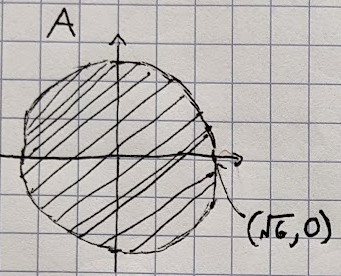
\includegraphics[width=12em]{media/A.png}
			\item $\{(x,y) \in \mathbb R^2 : x^2 + y^2 \leq 6\}$
		\end{enumerate}
	    \item $B$
	    \begin{enumerate}
			\item \phantom{ }
			
			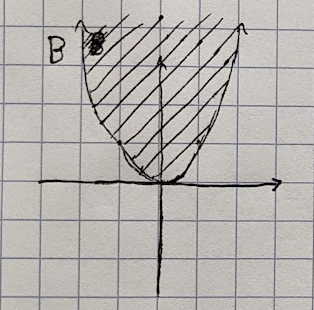
\includegraphics[width=12em]{media/B.png}
			\item $\{(x,y) \in \mathbb R^2 : y \geq x^2\}$
		\end{enumerate}

		\phantom{ }

	    \item $A \cup B$
	    \begin{enumerate}
			\item \phantom{ }
			
			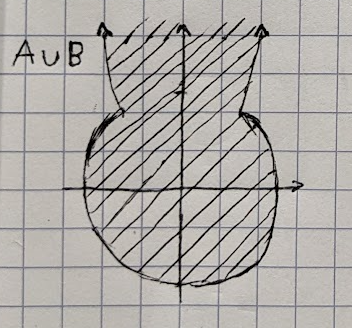
\includegraphics[width=12em]{media/A_cup_B.png}
			\item $\{(x,y) \in \mathbb R^2 : x^2 + y^2 \leq 6 \text{ or } y \geq x^2\}$
		\end{enumerate}
	    \item $A \cap B$
	    \begin{enumerate}
			\item \phantom{ }
			
			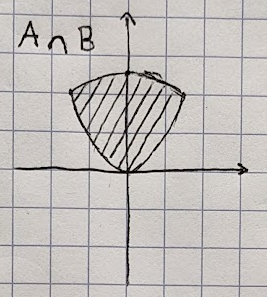
\includegraphics[width=11em]{media/A_cap_B.png}
			\item $\{(x,y) \in \mathbb R^2 : x^2 + y^2 \leq 6 \text{ and } y \geq x^2\}$
		\end{enumerate}
		\item $A - B$
	    \begin{enumerate}
			\item \phantom{ }
			
			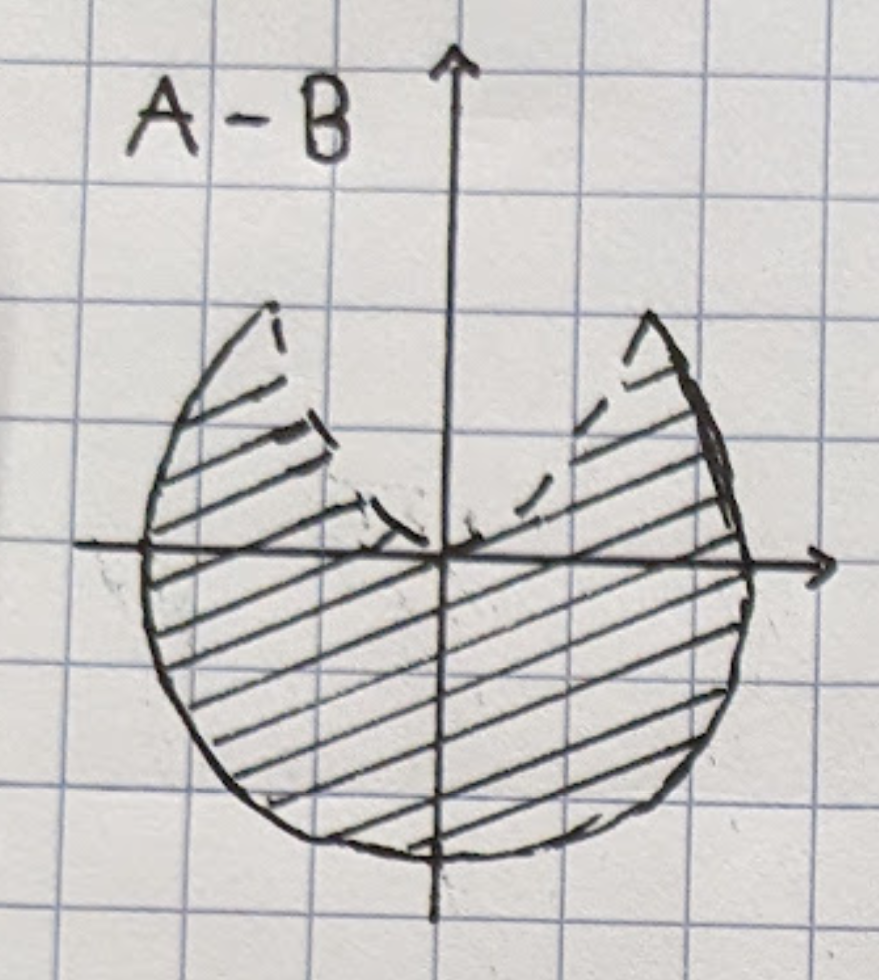
\includegraphics[width=11em]{media/A-B.png}
			\item $\{(x,y) \in \mathbb R^2 : x^2 + y^2 \leq 6 \text{ and } y < x^2\}$
		\end{enumerate}
		\item $B - A$
	    \begin{enumerate}
			\item \phantom{ }
			
			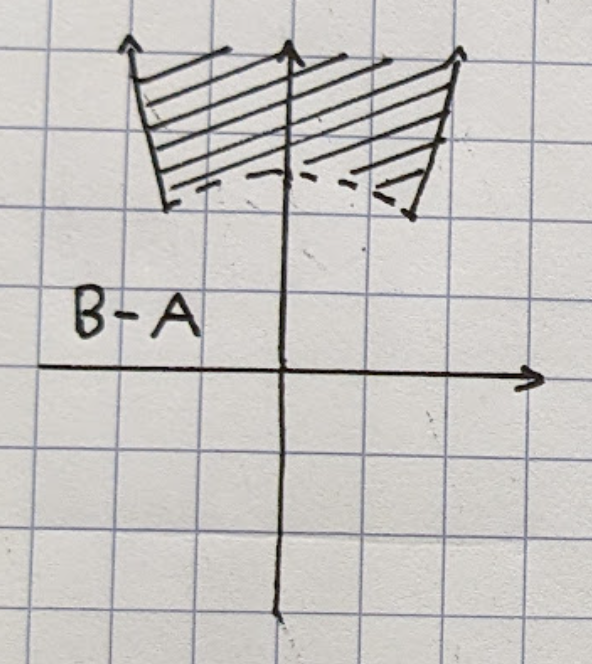
\includegraphics[width=10em]{media/B-A.png}
			\item $\{(x,y) \in \mathbb R^2 : x^2 + y^2 > 6 \text{ and } y \geq x^2\}$
		\end{enumerate}
		\item $\overline A$
	    \begin{enumerate}
			\item \phantom{ }
			
			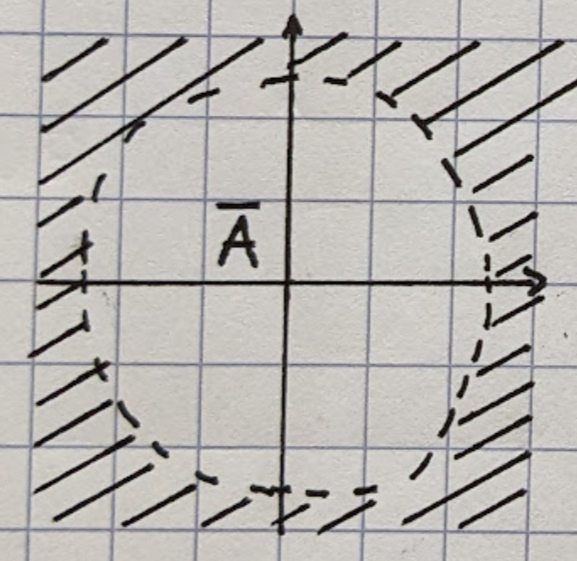
\includegraphics[width=12em]{media/overlineA.png}
			\item $\{(x,y) \in \mathbb R^2 : x^2 + y^2 > 6\}$
		\end{enumerate}
		\item $\overline B$
	    \begin{enumerate}
			\item \phantom{ }
			
			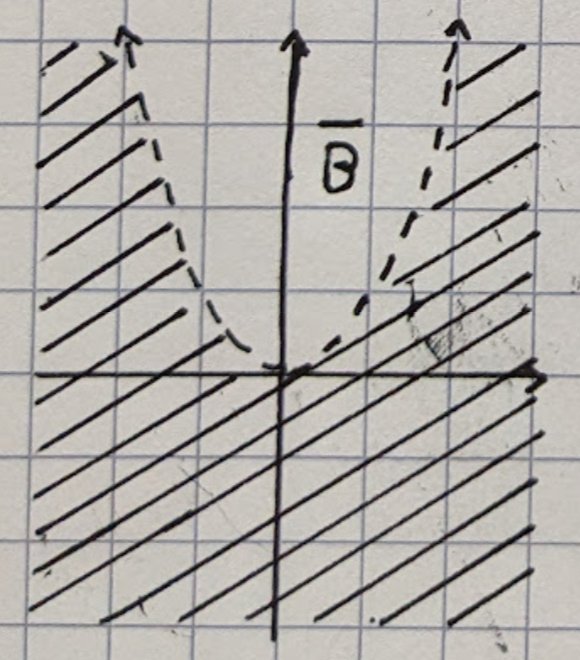
\includegraphics[width=11em]{media/overlineB.png}
			\item $\{(x,y) \in \mathbb R^2 : y < x^2\}$
		\end{enumerate}
		\item $\overline{A \cup B}$
	    \begin{enumerate}
			\item \phantom{ }
			
			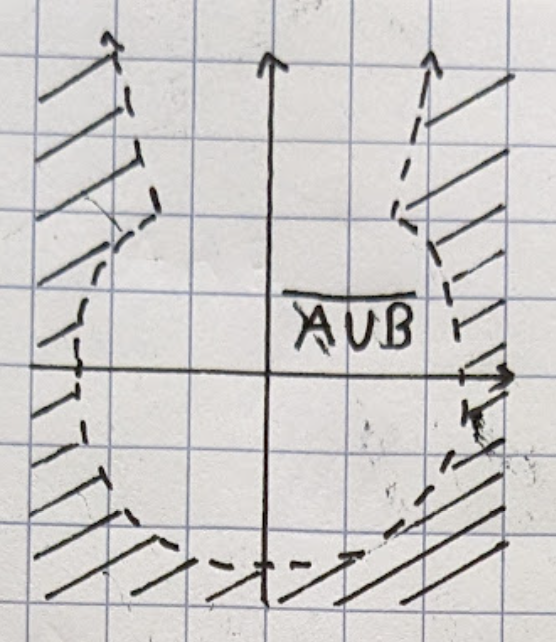
\includegraphics[width=12em]{media/overlineA_cup_B.png}
			\item $\{(x,y) \in \mathbb R^2 : x^2 + y^2 > 6 \text{ and } y < x^2\}$
		\end{enumerate}
		\item $\overline{A \cap B}$
		\begin{enumerate}
			\item \phantom{ }
			
			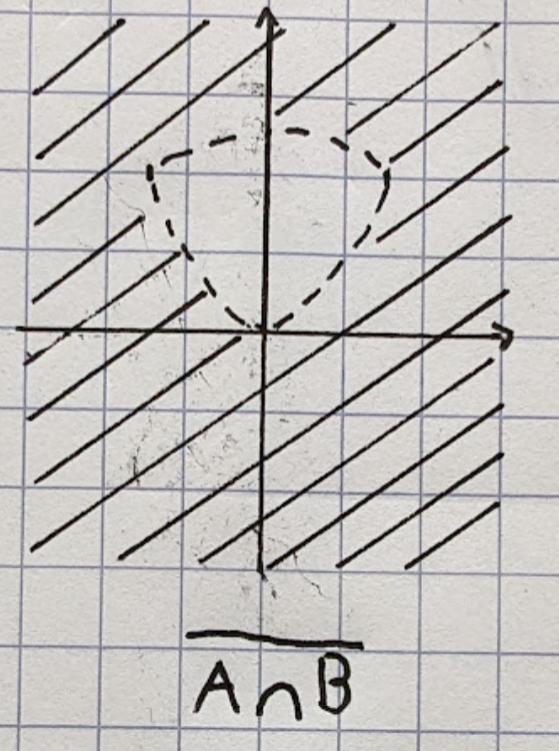
\includegraphics[width=12em]{media/overlineA_cap_B.png}
			\item $\{(x,y) \in \mathbb R^2 : x^2 + y^2 > 6 \text{ or } y < x^2\}$
		\end{enumerate}
    \end{itemize}
\end{soln}

\phantom{ }

\phantom{ }

\phantom{ }

\phantom{ }

\phantom{ }

\phantom{ }

\phantom{ }
%%%%%%%%%%%%%%%%%%%%%%%%%%%%%%%%%%%%%%%%%%%%%%%%%%%%%%%%%%%%%%%%%%%%%%%%%%%%%%
\begin{problem}
	For each $\alpha\in\R$, define $A_\alpha = \{(x,\alpha x)\in\R^2\,:\, -1\leq x\leq 1\}$.
	\begin{enumerate}
		\item Describe in words the set $A_\pi$.
		\item Describe $\displaystyle\bigcup_{\alpha\in\R} A_\alpha$ and $\displaystyle\bigcap_{\alpha\in\R} A_\alpha$ in set-builder notation.
	\end{enumerate}
\end{problem}

\begin{soln}
	\phantom{ }
	\begin{enumerate}
		\item This set can be described as a linear function with a slope of $\pi$ and a y-intercept of $0$
		on the closed interval $[-1,1]$.

		\item $\displaystyle\bigcup_{\alpha\in\R} A_\alpha = \{(x,y) \in \mathbb R^2 : x \in  [-1,1], \exists k (y = kx)\}$
		
		% $\{(x,y) \in \mathbb R^2 : x \in  [-1,0) \text{ or } x \in (0,1]\} \cup {(0,0)}$
		
		\noindent $\displaystyle\bigcap_{\alpha\in\R} A_\alpha = \{(0,0)\}$

		
	\end{enumerate}
	
\end{soln}
%%%%%%%%%%%%%%%%%%%%%%%%%%%%%%%%%%%%%%%%%%%%%%%%%%%%%%%%%%%%%%%%%%%%%%%%%%%%%%
\end{document}